\chapter{Preliminary Concepts and Formulations}\label{chp:preliminary-concepts}

In this chapter, we introduce the fundamental concepts necessary for understanding this thesis. The basic notation and definitions are presented in Section~\ref{sec:not-e-def}. In this work, we employ basic concepts from Combinatorial Optimization, which are assumed to be known. If the reader deems a review necessary, we recommend the textbook by Nemhauser and Wolsey~\cite{Nemhauser}, which covers this topic with a focus on \gls{ilp}, one of the main tools used in this work. 

Basic concepts related to graph theory are also assumed to be known. Should the reader require a refresher, the material can be found in standard textbooks on the subject, such as Diestel~\cite{diestel:2005}. 

The mathematical models are presented in Sections~\ref{sec:dmfm-pma} and~\ref{sec:ab-pma}. Section~\ref{sec:rel-lagrangiana} provides a description of the functioning and application of Lagrangian relaxation, one of the main approaches employed in this work. Finally, in Sections~\ref{sec:metaheuristic} and~\ref{subsec:brkga}, we present a general discussion on metaheuristics.

\section{Notations and Definitions} \label{sec:not-e-def}

Let $G = (V, A)$ be a weighted and directed graph, where $V = \{1, \dots, n\}$ is the set of vertices and $A = \{(u, v) : u \text{ and } v \in V, u \neq v\}$ is the set of $m$ arcs. In each arc, the first vertex is the source and also the predecessor of the second vertex in the ordered pair, which is known as the destination.

For undirected graphs, the arc set $A$ can be replaced by the edge set $E$. A tree $T$, obtained from an undirected graph $G$, is a connected subgraph of $G$ that contains no cycles. In order for $T$ to be a spanning tree in $G$, the vertex set $V(T)$ must be equal to $V(G)$—that is, all vertices of the graph must be part of the tree. An arborescence, or rooted tree, is a directed graph in which exactly one vertex, say $s$, has in-degree 0, and no vertex has in-degree greater than 1, such that all vertices of the graph are reachable from the root $s$.

We now present a formal definition of the \gls{pma}. Let a VANET network be represented as a weighted directed graph $G = (V, A)$. Each arc in $G$ has three associated \gls{qos} metrics: \textit{delay}, \textit{jitter}, and bandwidth. The input to the \gls{pma} is defined as the tuple ($G(V, A), \lambda, \xi, \omega, s, D, \Delta_{d}, \Delta_{j}, \Delta_{v}, \Phi$), where:

\begin{itemize}
    \item $G = (V, A)$ is a weighted directed graph;
    \item $\lambda_{ij} : A \rightarrow \mathbb{N}$ is a function that returns the \textit{delay} value for each arc $(i, j) \in A$;
    \item $\xi_{ij} : A \rightarrow \mathbb{N}$ is a function that returns the \textit{jitter} value for each arc $(i, j) \in A$;
    \item $\omega_{ij} : A \rightarrow \mathbb{N}$ is a function that returns the bandwidth value for each arc $(i, j) \in A$;
    \item $s \in V$ is defined as the root;
    \item $D$ is the set of terminal vertices, such that $D \subseteq (V \backslash \{s\})$;
    \item $\Delta_{d}$ is a constant indicating the end-to-end \textit{delay} limit allowed in the path from $s$ to each vertex in $D$;
    \item $\Delta_{j}$ is a constant indicating the \textit{jitter} limit allowed in the path from $s$ to each vertex in $D$;
    \item $\Delta_{v}$ is a constant indicating the limit of end-to-end delay variation between all pairs of paths from $s$ to any vertex in $D$;
    \item $\Phi$ is a constant indicating the minimum required bandwidth for an arc to be eligible for inclusion in a solution;
\end{itemize}

In this section, we define the objective and operational constraints that govern the routing of spraying vehicles for dengue control. The effectiveness of insecticide application is maximized when spraying occurs at dawn or just before sunset. During these periods, a thermal inversion keeps the insecticide at lower altitudes, where mosquitoes are typically found~\citep{MS}. Once a spraying vehicle begins to service a city block, it must sequentially cover all surrounding edges in a clockwise direction. \textcolor{red}{The traversal ensures that the insecticide fog forms a continuous barrier, preventing mosquitoes from escaping. The clockwise direction is due to real operational factors, as the nebulizer equipment points to the right side of the vehicle.
Figure~\ref{fig:instance_digraph_fumace_car} shows an example of a map,
with four blocks to service, and Figure~\ref{fig:route_fumace_car} presents a spraying route for these blocks where the nebulizer is activated in the black dots and follows the direction of the arrow, starts by serving Block 2, goes to Blocks 1, 3 and 4, respectively.
}

\begin{figure}[h!]
  \begin{minipage}[c]{.49\textwidth}
    \centering
    \subfloat[A CBRP instance digraph.]{\label{fig:instance_digraph_fumace_car}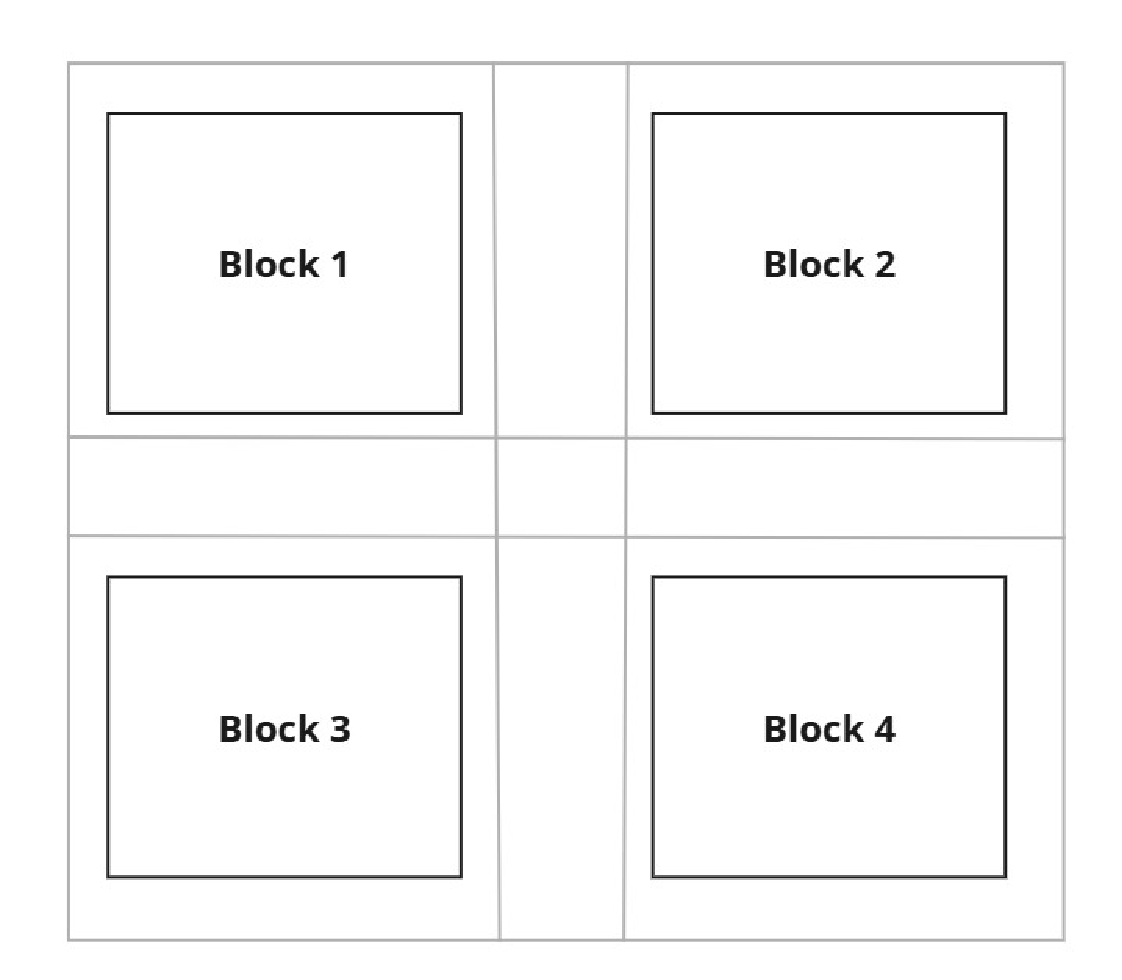
\includegraphics[width=5cm, height=5cm]{cbrp-instance.pdf}}
  \end{minipage}%
  \begin{minipage}[c]{.49\textwidth}
    \centering
    \subfloat[A spraying vehicle route covering four city blocks.]{\label{fig:route_fumace_car}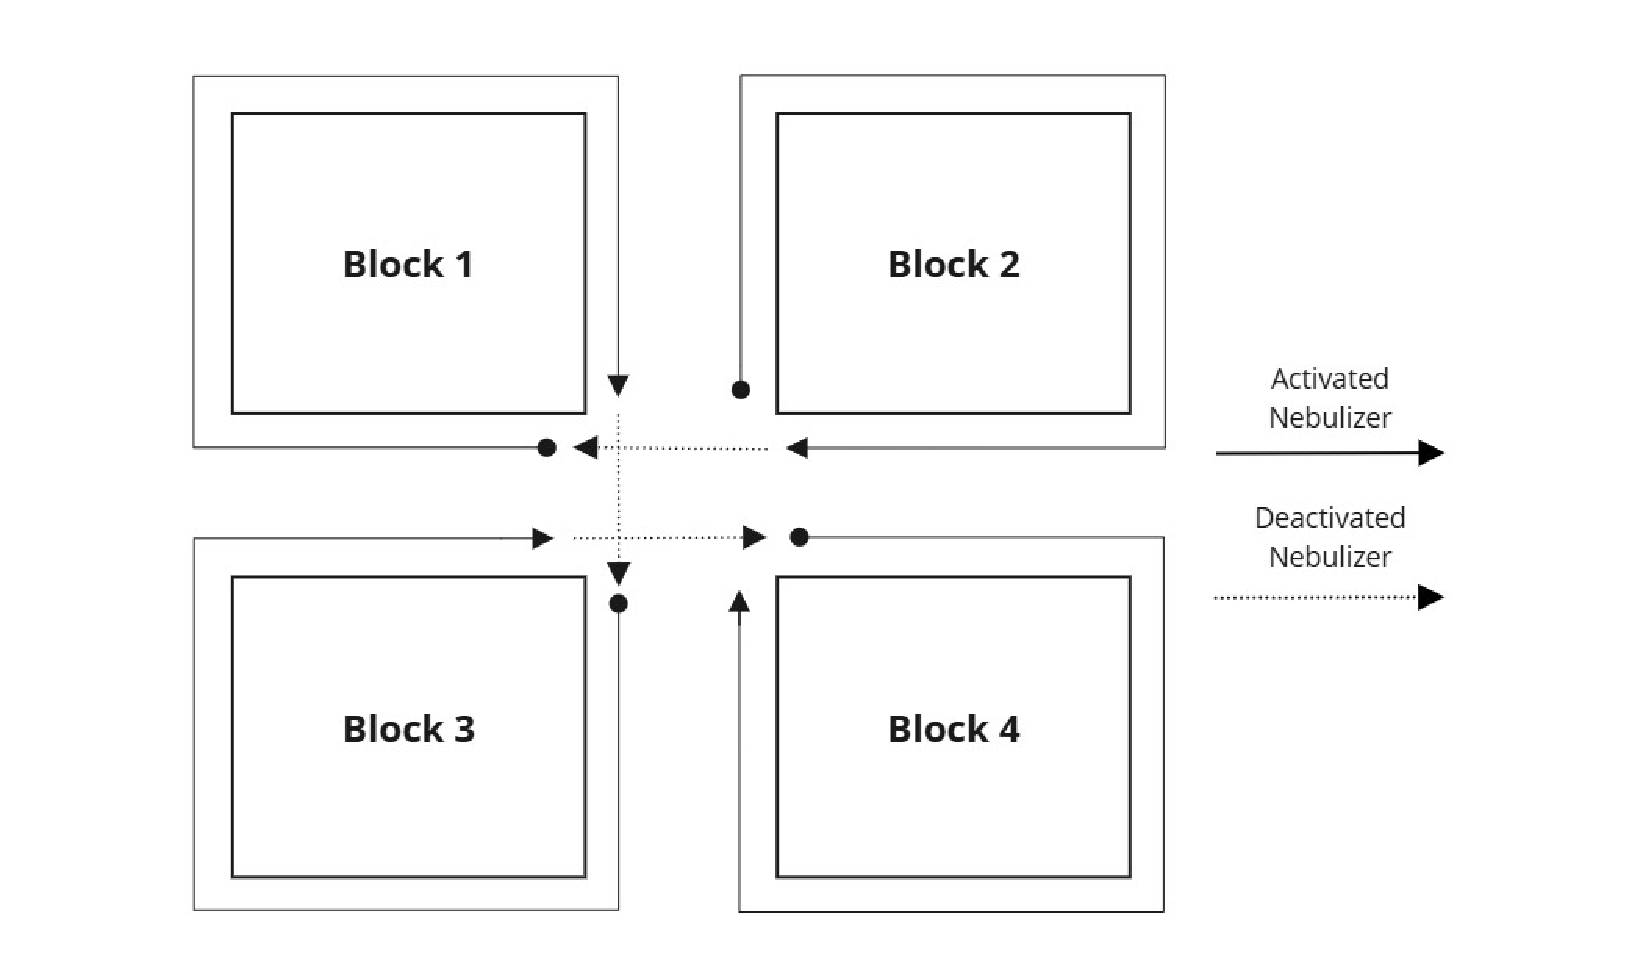
\includegraphics[width=8cm, height=5cm]{nebulizer-activated.pdf}}
  \end{minipage}
  \caption{\label{fig:route-ex} CBRP example.}
\end{figure}

The CBRP is introduced as a general framework for addressing the routing of spraying vehicles and other city block servicing problems. The objective of the CBRP is to determine an optimal traversal that services a subset of blocks within a network, maximizing the total collected benefit from each serviced block. We define the CBRP as follows. Consider a planar-oriented graph $D(V,A)$ representing a street network, where each arc $a \in A$ has a deadheading time $t_a \geqslant 0$ and a service time $t^{'}_a$ such that $t_a \leqslant t^{'}_a$. There is a set of city blocks $B = \{b : b \subseteq A\}$, where each block $b$ has an associated prize $p_b$ that can be collected by servicing all its surrounding arcs and the notation $t^{'}_b$ is used to represent the sum of the service time for all arcs $b$. A vehicle traverses the graph $D$ following a route that can serve a subset of blocks within a given time limit $T$. This work considers two types of solution routes, depending on whether the vertices can be visited more than once: \textit{Walk-based route}, in which any vertex (or arc) can be visited multiple times; and \textit{Path-based route}, in which no vertex appears more than once. An optimal route (walk or path) is one that maximizes the total prize collected from the serviced blocks while respecting the vehicle time limit $T$.

We now present key properties of the CBRP. First, we observe that once a block starts being serviced at a given node, it must be fully encircled before the vehicle moves to another block. This leads to the following properties.

\begin{property}
\label{claim:core_insight}
A block can be serviced if at least one of its nodes is visited.
\end{property}

From Property~\ref{claim:core_insight}, when formulating the problem, it is not necessary to explicitly require the vehicle to completely traverse a block's perimeter in order to count it as serviced. Instead, servicing can be achieved by visiting at least one node within the block and accounting for the corresponding service time. 

\Cref{fig:servicing_block_no_surrounding_strategy} illustrates an example of this strategy, where servicing is achieved without requiring a full traversal of the block’s perimeter.

\begin{figure}[ht!]
  \centering
  \begin{subfigure}{.3\textwidth}
    \centering
    \begin{tikzpicture}[>=latex, scale=.8]
      % nodes
      % block A
      \coordinate (A1) at (3, 2);
      \coordinate (A2) at (4, 1);
      \coordinate (A3) at (2, 1);
      \coordinate (BorderA1) at (3, 2.1);
      \coordinate (BorderA2) at (4.2, 0.9);
      \coordinate (BorderA3) at (1.8, 0.9);
      % block B
      \coordinate (B1) at (2, 3);
      \coordinate (B2) at (1, 3);
      \coordinate (B3) at (1, 4);
      \coordinate (B4) at (2, 4);
      \coordinate (BorderB1) at (2.1, 2.9);
      \coordinate (BorderB2) at (0.9, 2.9);
      \coordinate (BorderB3) at (0.9, 4.1);
      \coordinate (BorderB4) at (2.1, 4.1);
      % block C
      \coordinate (C1) at (4, 3);
      \coordinate (C2) at (4, 4);
      \coordinate (C3) at (5, 4);
      \coordinate (C4) at (5, 3);
      \coordinate (BorderC1) at (3.9, 2.9);
      \coordinate (BorderC2) at (3.9, 4.1);
      \coordinate (BorderC3) at (5.1, 4.1);
      \coordinate (BorderC4) at (5.1, 2.9);
      % blocks
      \def\blockA{A1, A2, A3}
      \def\blockB{B1, B2, B3, B4}
      \def\blockC{C1, C2, C3, C4}
      % arcs
      \def\arcs{%
        BorderA1 BorderB1
        BorderB1 BorderA1
        BorderB1 BorderC1
        BorderC1 BorderB1
        % block A
        BorderA1 BorderA2
        BorderA2 BorderA1
        BorderA2 BorderA3
        BorderA3 BorderA2
        BorderA3 BorderA1
        BorderA1 BorderA3
        % block B
        BorderB1 BorderB2
        BorderB2 BorderB3
        BorderB3 BorderB4
        BorderB4 BorderB1
        BorderB2 BorderB1
        BorderB3 BorderB2
        BorderB4 BorderB3
        BorderB4 BorderB1
        % block C
        BorderC1 BorderC2
        BorderC2 BorderC3
        BorderC3 BorderC4
        BorderC4 BorderC1
        BorderC2 BorderC1
        BorderC3 BorderC2
        BorderC4 BorderC3
        BorderC1 BorderC4
      }
      \readarray\arcs\Arcs[15,2]
      % print arcs
      \drawArcs{\Arcs}{\ArcsROWS}{->, gray!20, to path={-| (\tikztotarget)}}
      % block 1
      \drawBlock{A1}{\blockA}{red!50};
      %block 2
      \drawBlock{B1}{\blockB}{black!50};
      %block 3
      \drawBlock{C1}{\blockC}{yellow!50};
    \end{tikzpicture}
    \caption{Instance example.}
    \label{fig:three_street_blocks_instance}
  \end{subfigure}
  \begin{subfigure}{.3\textwidth}
    \centering
    \begin{tikzpicture}[>=latex, scale=.8]
      % nodes
      % block A
      \coordinate (A1) at (3, 2);
      \coordinate (A2) at (4, 1);
      \coordinate (A3) at (2, 1);
      \coordinate (BorderA1) at (3, 2.1);
      \coordinate (BorderA2) at (4.2, 0.9);
      \coordinate (BorderA3) at (1.8, 0.9);
      % block B
      \coordinate (B1) at (2, 3);
      \coordinate (B2) at (1, 3);
      \coordinate (B3) at (1, 4);
      \coordinate (B4) at (2, 4);
      \coordinate (BorderB1) at (2.1, 2.9);
      \coordinate (BorderB2) at (0.9, 2.9);
      \coordinate (BorderB3) at (0.9, 4.1);
      \coordinate (BorderB4) at (2.1, 4.1);
      % block C
      \coordinate (C1) at (4, 3);
      \coordinate (C2) at (4, 4);
      \coordinate (C3) at (5, 4);
      \coordinate (C4) at (5, 3);
      \coordinate (BorderC1) at (3.9, 2.9);
      \coordinate (BorderC2) at (3.9, 4.1);
      \coordinate (BorderC3) at (5.1, 4.1);
      \coordinate (BorderC4) at (5.1, 2.9);
      % blocks
      \def\blockA{A1, A2, A3}
      \def\blockB{B1, B2, B3, B4}
      \def\blockC{C1, C2, C3, C4}
      % arcs
      \def\nonSprayingArcs{%
        BorderA1 BorderB1
        BorderB1 BorderC1
      }
      \readarray\nonSprayingArcs\NonSprayingArcs[2,2]
      % spraying arcs
      \def\arcsSpraying{%
        % block A
        BorderA1 BorderA2
        BorderA2 BorderA3
        BorderA3 BorderA1
        % block B
        BorderB1 BorderB2
        BorderB2 BorderB3
        BorderB3 BorderB4
        BorderB4 BorderB1
        % block C
        BorderC1 BorderC2
        BorderC2 BorderC3
        BorderC3 BorderC4
        BorderC4 BorderC1
      }
      \readarray\arcsSpraying\ArcsSpraying[11,2]
      % print arcs
      \drawArcs{\NonSprayingArcs}{\NonSprayingArcsROWS}{dashed, ->}
      \drawArcs{\ArcsSpraying}{\ArcsSprayingROWS}{->, to path={-| (\tikztotarget)}}
      % block 1
      \drawBlock{A1}{\blockA}{red!50};
      %block 2
      \drawBlock{B1}{\blockB}{black!50};
      %block 3
      \drawBlock{C1}{\blockC}{yellow!50};
      %lines
      % \filldraw[black] (BorderA1) circle (1pt);
    \end{tikzpicture}
    \caption{Explicit block servicing.}
    \label{fig:three_street_blocks_route_surrounding}
  \end{subfigure}
  \begin{subfigure}{.3\textwidth}
    \centering
    \begin{tikzpicture}[>=latex, scale=.8]
      % nodes
      % block A
      \coordinate (A1) at (3, 2);
      \coordinate (A2) at (4, 1);
      \coordinate (A3) at (2, 1);
      \coordinate (BorderA1) at (3, 2.1);
      \coordinate (BorderA2) at (4.2, 0.9);
      \coordinate (BorderA3) at (1.8, 0.9);
      % block B
      \coordinate (B1) at (2, 3);
      \coordinate (B2) at (1, 3);
      \coordinate (B3) at (1, 4);
      \coordinate (B4) at (2, 4);
      \coordinate (BorderB1) at (2.1, 2.9);
      \coordinate (BorderB2) at (0.9, 2.9);
      \coordinate (BorderB3) at (0.9, 4.1);
      \coordinate (BorderB4) at (2.1, 4.1);
      % block C
      \coordinate (C1) at (4, 3);
      \coordinate (C2) at (4, 4);
      \coordinate (C3) at (5, 4);
      \coordinate (C4) at (5, 3);
      \coordinate (BorderC1) at (3.9, 2.9);
      \coordinate (BorderC2) at (3.9, 4.1);
      \coordinate (BorderC3) at (5.1, 4.1);
      \coordinate (BorderC4) at (5.1, 2.9);
      % blocks
      \def\blockA{A1, A2, A3}
      \def\blockB{B1, B2, B3, B4}
      \def\blockC{C1, C2, C3, C4}
      % arcs
      \def\arcs{%
        BorderA1 BorderB1
        BorderB1 BorderC1
      }
      \readarray\arcs\Arcs[2,2]
      % print arcs
      \drawArcs{\Arcs}{\ArcsROWS}{dashed, ->}
      % block 1
      \drawBlock{A1}{\blockA}{red!50};
      %block 2
      \drawBlock{B1}{\blockB}{black!50};
      %block 3
      \drawBlock{C1}{\blockC}{yellow!50};
      %lines
      \filldraw[black] (BorderA1) circle (1pt);
    \end{tikzpicture}
    \caption{Implicit block servicing.}
    \label{fig:three_street_blocks_route_one_node_visit}
  \end{subfigure}
  \caption{Strategies for servicing blocks.}
  \label{fig:servicing_block_no_surrounding_strategy}
\end{figure}


Assuming the implicit servicing of a block as allowed by Property~\ref{claim:core_insight}, additional properties can be established concerning optimal solutions. Let $V_B = \bigcup_{b \in B} V(b)$ be the set of nodes belonging to some city block, and let $S^{*} = (v_1, ..., v_n)$ represent an optimal route.